\documentclass[compress]{ctexbeamer}

\usepackage{thumbpdf}
\usepackage{wasysym}
\usepackage{ucs}
\usepackage[utf8]{inputenc}
\usepackage{pgf,pgfarrows,pgfnodes,pgfautomata,pgfheaps,pgfshade}
\usepackage{pgfpages}
\usepackage{verbatim}
\usepackage{fancyvrb}
\usepackage{multimedia}
\usepackage{subcaption}
\usepackage{ulem}
\usepackage{textcomp}
\usepackage{tikz}

\usepackage{listings}

\usepackage{epigraph}
\setlength{\epigraphwidth}{.8\textwidth}

\usepackage{DejaVuSansMono}

% Adjust the colours to fit your design
\definecolor{mainthemecolour}{rgb}{0.42,0.48,0.37}
\definecolor{mainthemecolourlight}{rgb}{0.63,0.72,0.57}
\definecolor{mainthemecolourstrong}{rgb}{0.40,0.68,0.18}
\definecolor{mid-gray}{gray}{0.7}

\definecolor{greenstrong}{rgb}{0.58,0.77,0.29}
\definecolor{redstrong}{rgb}{0.81,0.22,0.23}
\definecolor{fglisting}{gray}{0.3}
\definecolor{bglisting}{gray}{1}
\definecolor{fgshell}{gray}{1}
\definecolor{bgshell}{gray}{0.1}
\definecolor{bgshelllight}{gray}{0.8}


% Some in-code macros - a bit buggy, but useful
\newcommand{\hl}[1]{\textcolor{greenstrong}{\texttt{#1}}}
\newcommand{\hlErr}[1]{\textcolor{redstrong}{\texttt{#1}}}
\newcommand{\hlOk}[1]{\textcolor{green}{\texttt{#1}}}
\newcommand{\hlInv}[1]{\colorbox{bgshell}{\textcolor{fgshell}{\texttt{#1}}}}

\newcommand{\unhl}[1]{\textcolor{gray}{#1}}
\newcommand{\clda}[0]{$\textcolor{blue}{\lambda}$}
\newcommand{\carr}[0]{$\textcolor{purple}{\rightarrow}$}
\newcommand{\cbind}[0]{\textbf{\texttt{$>\!\!>\!\!=$}}}
\newcommand{\codedots}[0]{\textcolor{mid-gray}{...}}

\usetheme{elegance}

\lstnewenvironment{cxxcode}
    {\lstset
        { escapeinside={@}{@}
        , gobble=8
        , showstringspaces=false
        , basicstyle=\color{fglisting}
        , rulecolor=\color{mainthemecolourlight}
        }
    }
    {}

\lstnewenvironment{cxxcodebox}
    {\lstset
        { escapeinside={@}{@}
        , gobble=6
        , showstringspaces=false
        , basicstyle=\color{fglisting}
        , frame=lr
        , rulecolor=\color{mainthemecolourlight}
        }
    }
    {}

\lstnewenvironment{shellcode}
    {\lstset
        { escapeinside={@}{@}
        , gobble=7
        , showstringspaces=false
        , basicstyle=\color{fgshell}
        , backgroundcolor=\color{bgshell}
        }
    }
    {}


% Marking points to use in Tikz
\usetikzlibrary{arrows,shapes}
\newcommand{\tikzmark}[1]{\tikz[remember picture] \node[coordinate] (#1) {#1};}

% Fragile frames
\newenvironment{xframe}[1][]
  {\begin{frame}[fragile,environment=xframe,#1]}
  {\end{frame}}


\title{青春猪头少年不会梦到反代和 P2P}
\subtitle{在内网设备上搭建公网服务的方案和原理介绍}
\author{\footnotesize 浙江工业大学 精弘网络}

\institute{\color{white}
As always have a nice day!\\
https://github.com/zjutjh
} %
\date{\footnotesize\color{mainthemecolour} 2021.04.04 }



\begin{document}

\maketitle

\section{引入与前置知识}

\subsection{从搭建公网 Minecraft 服务器说起}

\begin{xframe}{搭建公网 Minecraft 服务器}
	假设有两个人 Alice 和 Bob,他们想要联机一起玩 Minecraft。\pause
	
	考虑以下两种情况:\\
	\begin{itemize}
		\item Alice 和 Bob 在同一个局域网
		\item Alice 和 Bob 不在同一个局域网
	\end{itemize}
\end{xframe}

\begin{xframe}{搭建公网 Minecraft 服务器}
	为什么不在同一个局域网时无法愉快的玩耍? \pause
	
	大致有以下原因:\\
	\begin{itemize}
%		\item 防火墙 (Firewall)
		\item IP 地址的动态分配 (DHCP)
		\item 网络地址转换 (NAT)
	\end{itemize}
\end{xframe}

% \begin{xframe}{防火墙 (Firewall)}
% 	一般来说,防火墙作为一种安全机制,用于监控入站和出站网络流量,并可根据一定的规则来决定是允许还是阻止特定流量。
% 	
% 	\begin{figure}[h]
% 		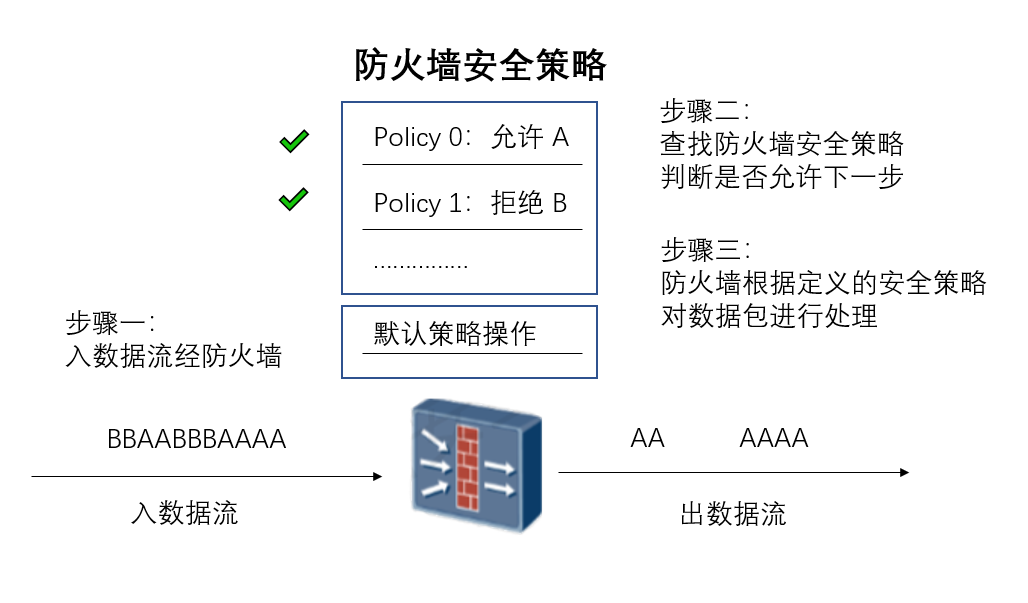
\includegraphics[width=200px]{1.png}
% 	\end{figure}
% 	\pause
% 	
% 	但当我们对外提供服务时,需要允许相应的数据包进入。\pause
% 	
% 	解决方案也相对比较简单,只需要调整防火墙的过滤规则即可。
% \end{xframe}

\begin{xframe}{IP 地址的动态分配 (DHCP)}
	IP 地址是用于区分不同主机的一种标识。通过IP地址,设备间可以互相通讯,如果没有IP地址,我们将无法知道哪个设备是发送方,无法知道哪个是接收方。\pause
	
	目前广泛使用的还是 IPv4 地址,它将这种标识定义为四字节的整数,通常用 4 个点分十进制来表示,例如 192.168.1.1。\pause
	
	入网设备长期使用一个固定的 IP 地址会使 IP 资源得不到有效利用。DHCP 通过在 IP 资源闲置的时候回收地址资源供其他用户使用,从而让有限的 IP 资源流动起来。
	
%	用户通常不会 24 小时都在使用网络,那么在你不使用网络的时候,IP 资源可以给其他用户使用,从而让有限的 IP 资源流动起来。
\end{xframe}

\begin{xframe}{IP 地址的动态分配 (DHCP)}
	但 DHCP 也给我们开服带来了一些问题,动态的地址会使得其他玩家无法长期通过一个确定的 IP 地址定位到你的服务器。\pause
	
	那么我们可以通过什么定位呢?\pause
	
	——域名和 DDNS 机制。
	
%   因为时间有限,无法展开讲这一部分的内容
	感兴趣的同学可以自行了解 DNS 和 DDNS 的原理和机制。\pause
%   可能以前折腾过 Minecraft 开服的同学可能会接触过花生壳(DDNS)、向日葵 / 蛤蟆吃(VPN 组网)

	DHCP 它显然给服务构建造成了不便,所以并不是所有 IP 地址都是动态分配的。事实上搭建公网服务的服务器大多具有确定的公网 IP 地址。
%   所以还是建议在公网服务器上搭建服务,这些问题说到底都是自己找的,别人本来就没想过你要在内网中搭建服务。
%   那么我们为什么要这么做呢?
%   我们可以想象,在自己的电脑上搭建 MC 服务器和租一台足以运行 MC 服务器的成本关系,这只是其中一个例子,其实有不少应用场景需要在自己的设备上搭建服务
%   比如在 NAS、树莓派,家里的个人云,要在户外访问(NAS)。
\end{xframe}

\begin{xframe}{网络地址转换 (NAT) —— NAT 的引入}
%	在不考虑保留地址等特殊地址的情形下,IPv4 的可用地址数大致为 $2^32$,大概 40 亿
	在 NAT 提出之前,每台入网设备都需要占用唯一的 IP 地址,而 IPv4 可用地址数\textbf{大概}只有 40 亿,在互联网发展到一定规模时已经无法适应实际需求了。\pause
%   当然有些同学可能有了解,地址更长的,为 16 字节 IPv6 也是一种解决方案,而且目前在不断推进。	
	
	而 NAT 提供了一种将内部 IP 地址和端口映射为外部相应 IP 地址和端口的方案,一定程度上解决了 IP 地址短缺的问题。
	(注:我们一般提到的 NAT 都是指动态的 NAPT,涉及端口转换)
	
%    注:我们一般提到的 NAT 其实都是 NAPT,涉及端口转换
\end{xframe}

\begin{xframe}{网络地址转换 (NAT) —— NAT 的原理}
%   我们来看一下在 NAT 下设备的上网方式:
	\begin{figure}[h]
		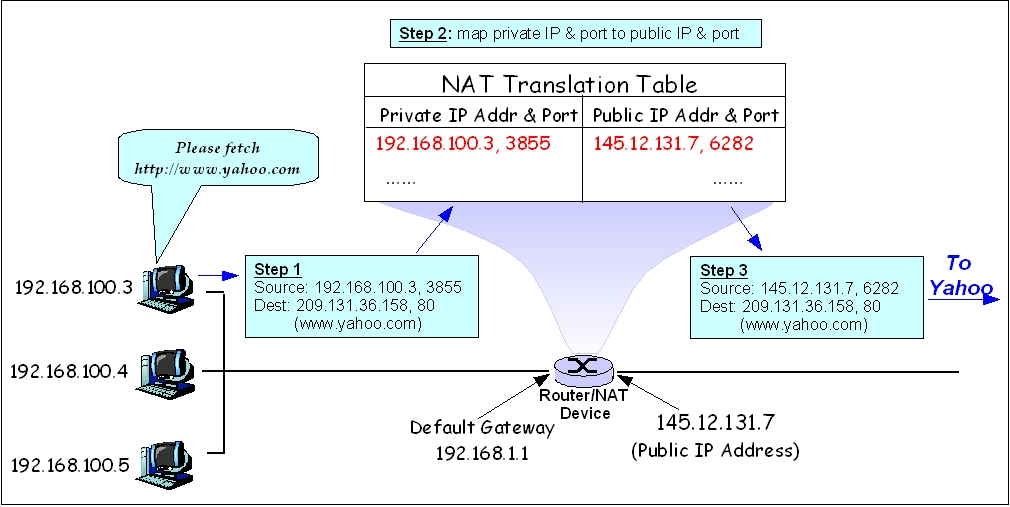
\includegraphics[width=300px]{Network_Address_Translation.jpg}
	\end{figure}
\end{xframe}

\begin{xframe}{网络地址转换 (NAT) —— NAT 对搭建服务的影响}
	同样为了端口资源的有效利用,NAT 的映射规则往往是动态的,如果超过一定时间没有使用,映射规则就会被删除。\pause
	
	而且 NAT 提供了一些安全规则,我们以其中一个比较常见的规则为例进行讨论:
	
	NAT 不会接受\textbf{来路不明}的数据,比如 Alice 并不会接受来自 Peter 的数据,除非 Alice 向 Peter 发过数据,这样 Peter 才会被 Alice 所在的 NAT 信任。\pause
%   当然不同类型的 NAT 可能情况不太一样,这个不是我们今天讨论的重点,有兴趣可以后续和我们进行交流。

%    回到 Alice 和 Bob 想要玩 Minecraft 的例子中,一般来讲,他们都是位于 NAT 之后的,那么按照前面的规则,他们两个无法直接建立连接。(为什么?)
%    那么我们怎样让他们愉快玩耍,这是我们要解决的问题。
	在这个规则下,如何让位于 NAT 之后的两个设备建立连接,是我们要解决的问题。
\end{xframe}

%\begin{xframe}{网络地址转换 (NAT)}
%	placeholder3
%\end{xframe}

\section{反向代理方案}

\subsection{原理和应用方案}

\begin{xframe}{反向代理方案}
%   两者都在 NAT 后面,基于前面的规则,我们无法让它们直接建立连接
%   如果有一个不在 NAT 后面的公网服务器作为中继服务器(代理),我们就可以对外提供服务。
%   不妨记两个为 Alice、Bob,服务器为 Server
	\begin{figure}[h]
		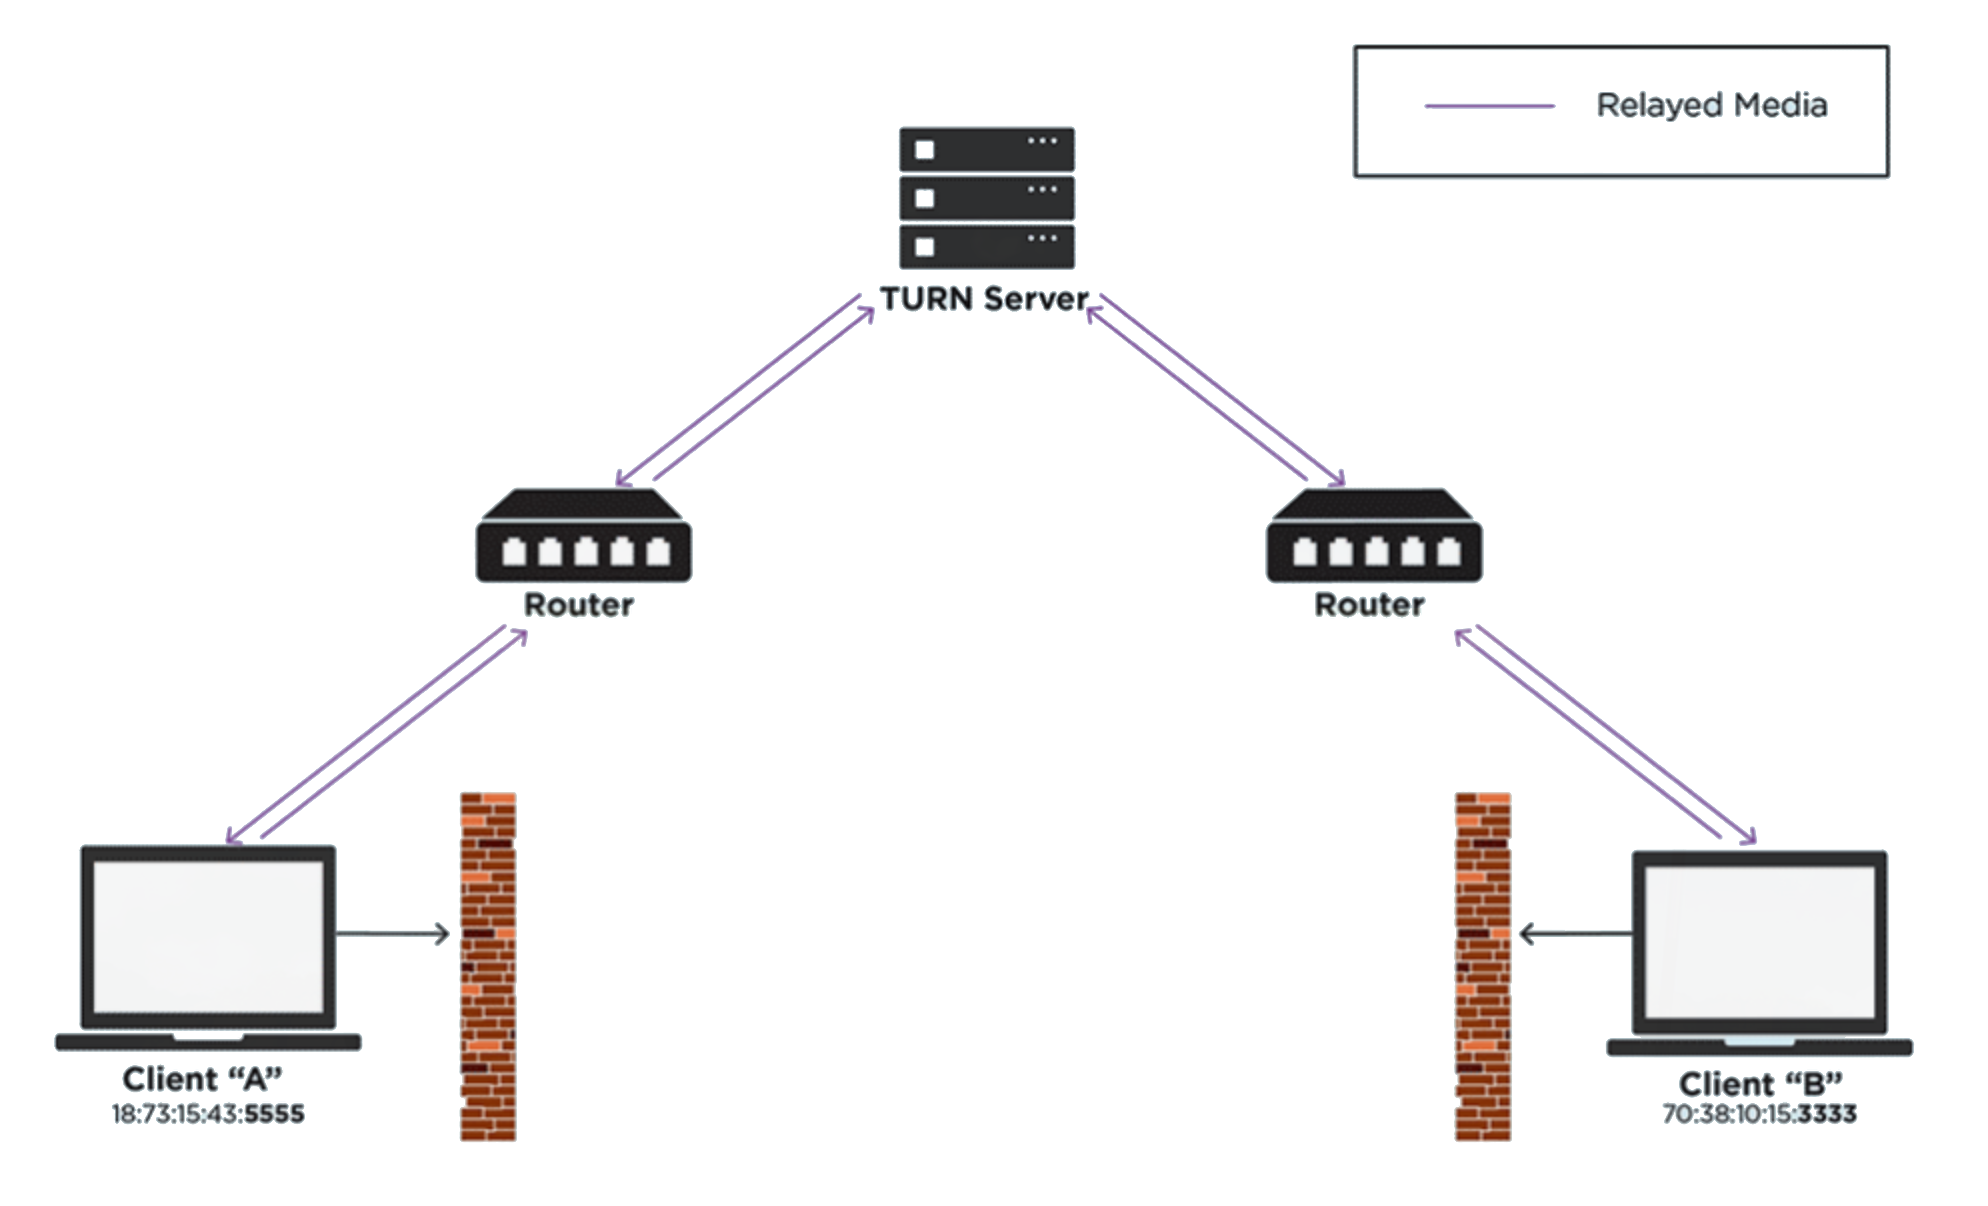
\includegraphics[width=300px]{2021-04-05_23-46.png}
	\end{figure}
\end{xframe}

\begin{xframe}{反向代理方案}
	现在 Alice 要开服务器,Alice 事先和 Server 约定好一个规则,并和 Server 建立连接,这样 Server 发给 Alice 的数据包就不会被丢弃(同时需要发送心跳包维护会话),把发送到特定端口的数据包都转发给 Alice。\pause
	
	于是通过 Server 中继流量,我们可以让 Alice 部署的服务在公网中可以被访问,于是远方的 Bob 就可以通过 Server 的地址加入服务器。
%   解释心跳包和前面提到的动态 NAT 机制。
%   问一下有没有理解
%   这个原理还是比较直观的。
%   它同时也隐藏了真正的服务地址。
	
	面向实际应用可以使用 ssh 隧道、frp、nginx 等方案。
\end{xframe}

\begin{xframe}{反向代理的其他应用}
	\begin{itemize}
		\item 为私有网络提供 NAT 穿透及外网发布服务
%   我们已经说过了
		\item 多域名跳转(vhost)
%   
		\item 负载均衡
%		\item 缓存服务器
	\end{itemize}
\end{xframe}

\begin{xframe}{多域名跳转 (vhost)}
	代理按照请求域名将请求数据分发到不同的内部服务器,分别处理。
	
	\begin{figure}[h]
		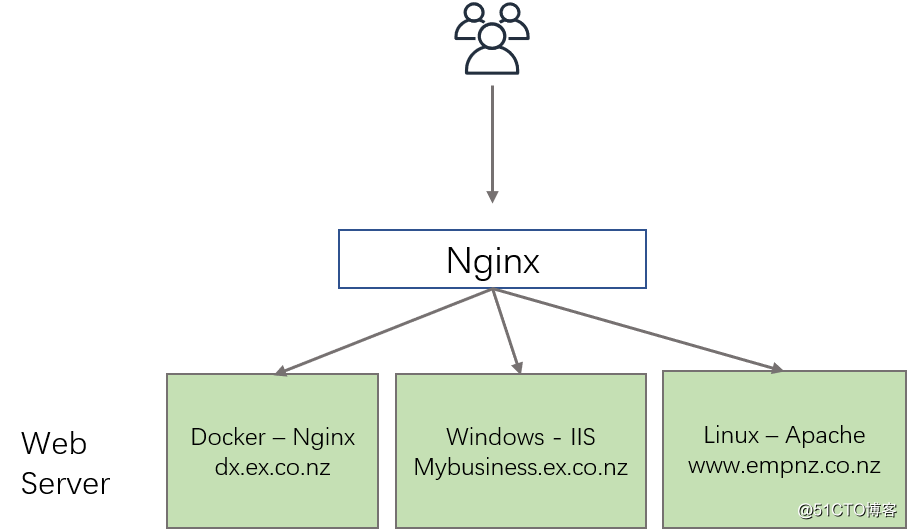
\includegraphics[width=200px]{6629cf9ff020bebc761bf6ba2302552f.png}
	\end{figure}
\end{xframe}

\begin{xframe}{负载均衡}
	反向代理服务器维护一个调度器,按照内部服务器的可用性将请求数据分发,分别处理,也可以很好的避免单点掉线的问题。
	
	\begin{figure}[h]
		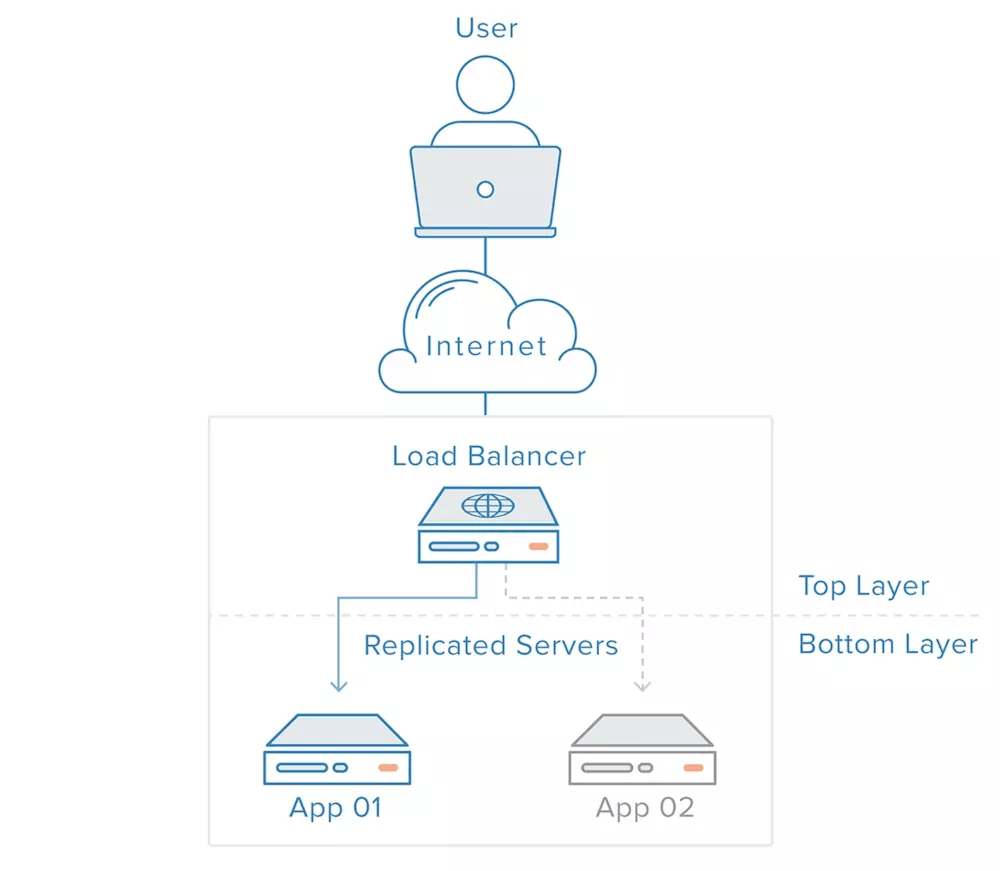
\includegraphics[width=180px]{k1k3EfHndY.png}
	\end{figure}
\end{xframe}

% \begin{xframe}{缓存服务器}
%	
%	\begin{figure}[h]
%		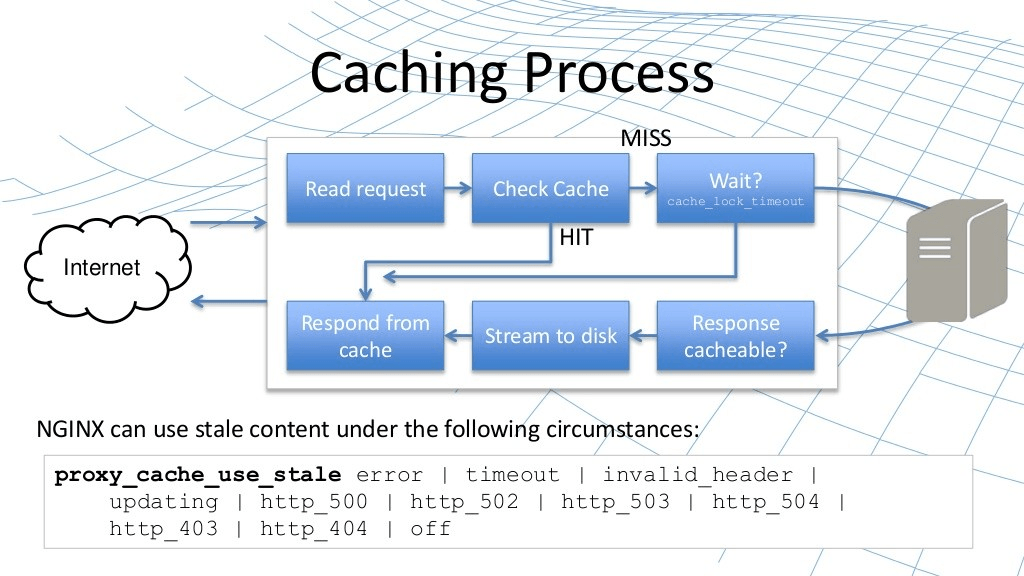
\includegraphics[width=250px]{zcxWo2c7JR.png}
%	\end{figure}
	
%   综合起来看,其实只是数据分发规则的不同,它可以完成很多事项,还是挺有意思的。
% \end{xframe}

%\begin{xframe}{网络地址转换 (NAT)}
%	placeholder2
%	1. 早期没有 NAT 的网络形态\\
%	2. 为什么会有 NAT 的提出(需要先介绍 IPv4 和其地址格式,作为出现地址短缺的原因和解决方案因为 IPv4 地址短缺,后面要提到 IPv6 的现状以及一些影响),在 NAT 下的上网形态\\
%	3. 为什么 NAT 给我们搭建公网服务造成了不便(当然可以直接在公网服务器上搭建服务,首先需要介绍公网服务器和其一般可访问性)\\
%	4. 回过去看,它其实和防火墙差不多,但是并不能像防火墙那样简单的设置(不过也有端口映射、UPnP、NAT-PMP 等方案,可以自行了解)\\
%	5. 告诉听众,下文的解决方案,主要是为了解决这个问题,P2P 方案在此基础上进行了一些扩展(图片、对比)\\
%	6. 讲到 P2P 还可以进行一定的延伸(SIP 协议)
%	7. (扩展)有了这些我们可以做什么,BT 下载的原理以及 DHT,简单介绍一下比特币的原理(neta 一下另外一组的内容)\\
%\end{xframe}

\section{P2P 方案}

\subsection{简单介绍原理和理论可行的方案}

\begin{xframe}{NAT 穿透}
%   反向代理方案在服务器比较可靠的情况下非常稳定,但是会消耗额外的带宽。而 
	NAT 穿透方案在多数情况下能够让 Alice 和 Bob 不经过中继服务器直接建立连接。
%   事实上国内带宽还是挺贵的。
%   如果能够不经过服务器,让 Alice 和 Bob 直连,那不仅延迟更小,而且还不会占用额外带宽,就很舒服了。
	
	\begin{figure}[h]
		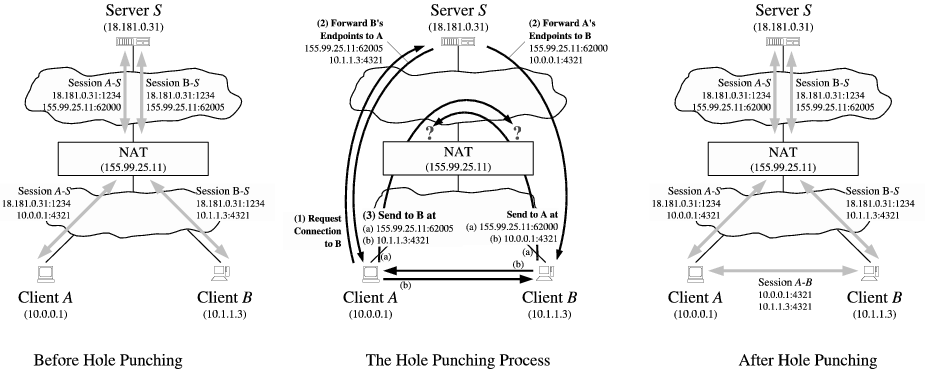
\includegraphics[width=300px]{img8.png}
	\end{figure}
\end{xframe}

\begin{xframe}{NAT 穿透}
	比较常见的方案是优先进行 NAT 穿透,如果无法 NAT 穿透就采用中继方案(比如 ICE 协议就是 STUN 和 TURN 的结合)。
	
	这样就实现了 P2P(点对点)的连接。\pause
	
	这种方式应用还是比较广泛的:
	
	\begin{itemize}
		\item IP 电话(VoIP,比如 Skype)
		\item P2P 应用(比如很多游戏的 P2P 对战模式) % 马里奥赛车之类的
		\item ...
	\end{itemize}
\end{xframe}

%\begin{xframe}{物理网络与重叠网络}
%	content...
%\end{xframe}

%\begin{xframe}{结构化去中心化网络}
%	content...
%\end{xframe}

\section{一些说明}

\subsection{细节和补充说明}

\begin{xframe}{关于 IPv6}
	IPv6 的网络地址空间很大,16 个字节,和 IPv4 的地址空间量级相差很大,于是内网和 NAT 的概念也就淡化了。
	
	又回到了 NAT 提出之前的模式,我们可以直接使用确定(但可能是动态的,因为 DHCP)的地址访问某个服务器。
	
	那么在 P2P 方面的扩展也会更加容易,点对点的连接建立不需要复杂的 NAT 穿透和中继过程。
	
\end{xframe}

\begin{xframe}{关于 IPv6}
	在 IPv6 下,没有 NAT 的安全机制,一些潜在的威胁,或者说\textbf{来路不明}的数据不会被拦截,并且可能借助本机某些端口存在的漏洞给设备带来威胁。\\
	
	因此我们要注意本机防火墙和安全规则的设立,以及具备一定的安全意识。
\end{xframe}

\begin{xframe}{关于 NAT 穿透}
	有一种比较特殊的 NAT 类型(对称型 NAT)无法使用前面讲到的 NAT 穿透方式。\\
	
	还有其他“NAT 穿透”的方案,比如端口映射、UPnP、NAT-PMP、DMZ 主机等,可以自行查阅相关资料。
	
\end{xframe}

\begin{xframe}{最后}
	考虑到主要目的是普及,而且时间有限,所以可能看起来像一个大杂烩,讲的东西比较多,但都比较浅略。\\
	
	希望能够帮助大家扩展一些对网络的理解,也希望能够引起大家对这部分知识的兴趣。\\
	
	Good Luck \& Have Fun!
\end{xframe}

\end{document}
